\chapter{Architectural Views for Your Suggestions to Improve the Existing System} \label{suggest}


\section{Context View}

% Refer to \textit{R\&W Chapter 16}. 

\subsection{Stakeholders’ uses of this view}

The key use of the Context View for the stakeholders of FarmBot is to ensure that the overall end-to-end solution indeed sensibly satisfies functionality requirements from a general viewpoint. The different stakeholders' uses of this view are as follows:
\begin{itemize}
    \item Developers: Use the context view in order to have a better picture of how the system fits into the overall application landscape. They use it to understand the interactions with external systems and entities. In addition to that, for further improvements to the system, they can better assess completeness, consistency, and coherence.
    \item End Users (Students, Researchers, Home Users, Artwork Creators): Use the context view in order to ensure that FarmBot is able to satisfy their requirements and that its scope is correct. Also, it enables them to learn how the data flows, the interactions are done throughout the FarmBot system, and what external entities or services are part of it.
    \item Ministry of Agriculture: Use the context view for auditing FarmBot as a system, see what external entities and services are used and where and how data flows.
\end{itemize}

\subsection{Context Diagram}

% \textbf{Context Diagram for your suggestion} should display all external entities that may interact with the system. This section should include a \textbf{Context Diagram and explanations} for the context diagram.

\begin{figure}[H]
    \centering
    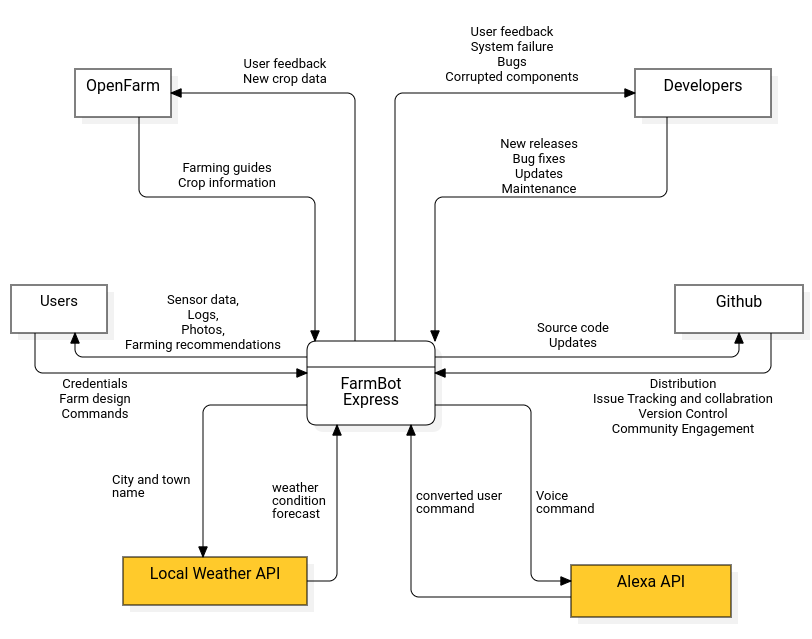
\includegraphics[width=1\textwidth]{Figures/SuggestedContextDiagram.png}
    \caption{Suggested Context Diagram for FarmBot}\label{fig:suggested_context}
\end{figure}

The suggested context diagram for FarmBot is shown in Figure \ref{fig:suggested_context}. The diagram shows the external entities that may interact with the system. It now includes \cite{weather_api} \textbf{Local Weather API} and \cite{alexa_api} \textbf{Alexa API} as new external system entities. The \textbf{Local Weather API} is used to get the weather information of the FarmBot location. The \textbf{Alexa API} is used to control the FarmBot using voice commands.

\subsection{External Interfaces}
% This section should include an \textbf{External Interfaces Class Diagram for your suggestion}. Descriptions of the operations given in the external interface class diagram should also be given. \textbf{You should aim for 2 external interfaces.}
\begin{figure}[H]
    \centering
    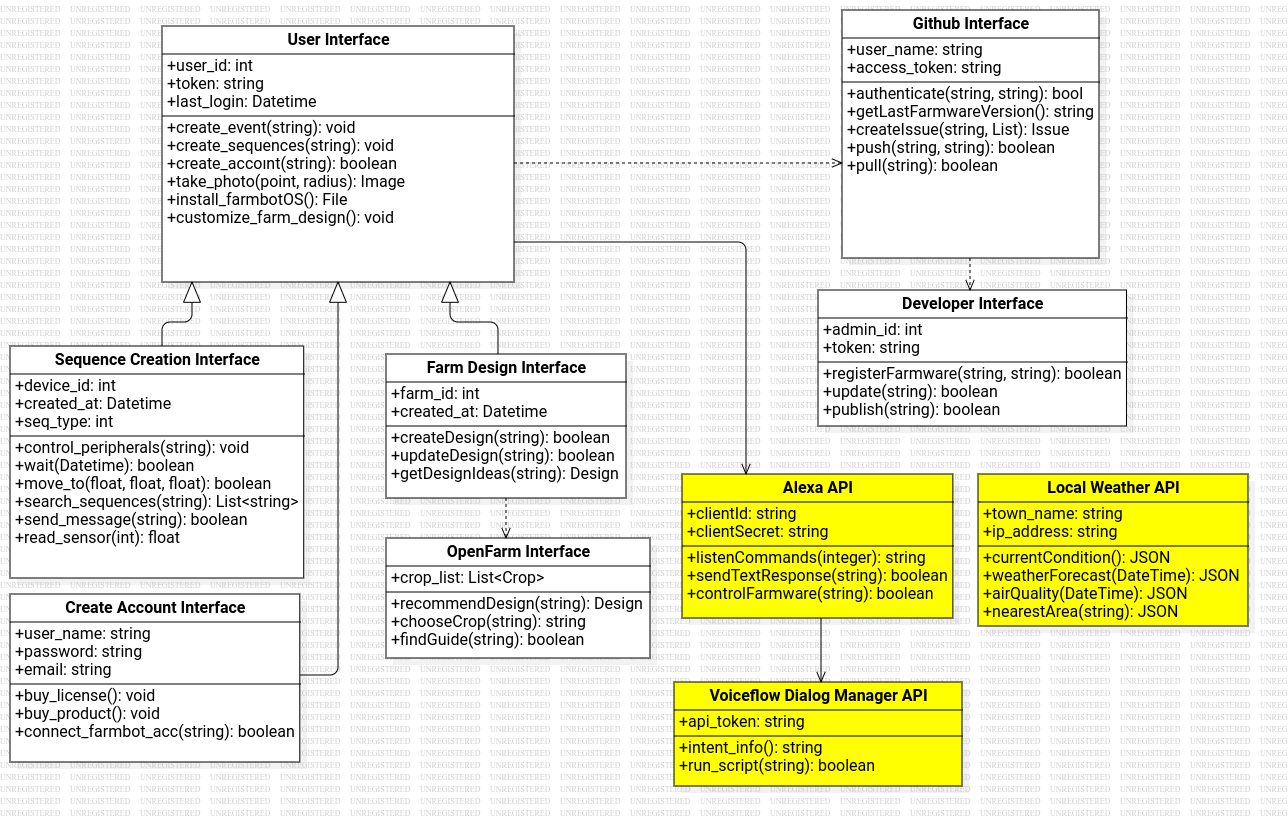
\includegraphics[width=1\textwidth]{Figures/SuggestedClassDiagram.png}
    \caption{Suggested External Interfaces Class Diagram for FarmBot}\label{fig:suggested_external_interfaces}
\end{figure}

The suggested external interfaces class diagram for FarmBot is shown in Figure \ref{fig:suggested_external_interfaces}. The diagram shows the external interfaces of the system. It now includes \textbf{Local Weather API} and \textbf{Alexa API} with \textbf{Voiceflow Dialog Manager API} as new external interfaces of the system.

\begin{itemize}
    \item \textbf{Local Weather API}: The system uses this API to get the weather information of the FarmBot location. The acquired data shows that current temperature, humidity, and weather conditions are used to adjust many functionalities of the FarmBot, such as watering the plants, turning on the lights, etc. Furthermore, the system can also use this data to predict the weather conditions for the upcoming days and adjust the FarmBot's schedule accordingly.
    \item \textbf{Alexa API}: The system uses this API to control the FarmBot using voice commands. The users can interact with the FarmBot using voice commands through the Alexa API. The system can understand the voice commands and execute the corresponding actions, such as watering the plants, turning on the lights, etc. The vocal commands of the users go into Alexa API; then it is redirected to the Voiceflow Dialog Manager API to understand the commands and execute the corresponding actions.
    \item \textbf{Voiceflow Dialog Manager API}: The system uses this API to understand the users' voice commands. Internally, it runs a voice recognition algorithm that understands the commands and executes the corresponding actions. The commands are then redirected to the FarmBot system to execute the corresponding actions.
\end{itemize}


\subsection{Interaction scenarios}
% This section includes \textbf{1 Activity Diagram} to show interaction sequences taking place over the external interfaces for \textbf{your suggestion.} Choose the most complex interaction for activity diagrams. They must differ from those in your \gls{srs} document.
The activity diagram for the voice command pipeline is shown in Figure~\ref{fig:suggested_activity}. The diagram shows the interaction sequences taking place over the external interfaces for the suggested system. The diagram illustrates the process of storing a voice command in the system, recognizing the command using the Voiceflow Dialog Manager API, and executing the corresponding action in the FarmBot system. The interaction starts with the user issuing a voice command through the Alexa API. The command is then processed by the Voiceflow Dialog Manager API, which recognizes the command and sends it to the FarmBot system for execution.

\begin{figure}[H]
    \centering
    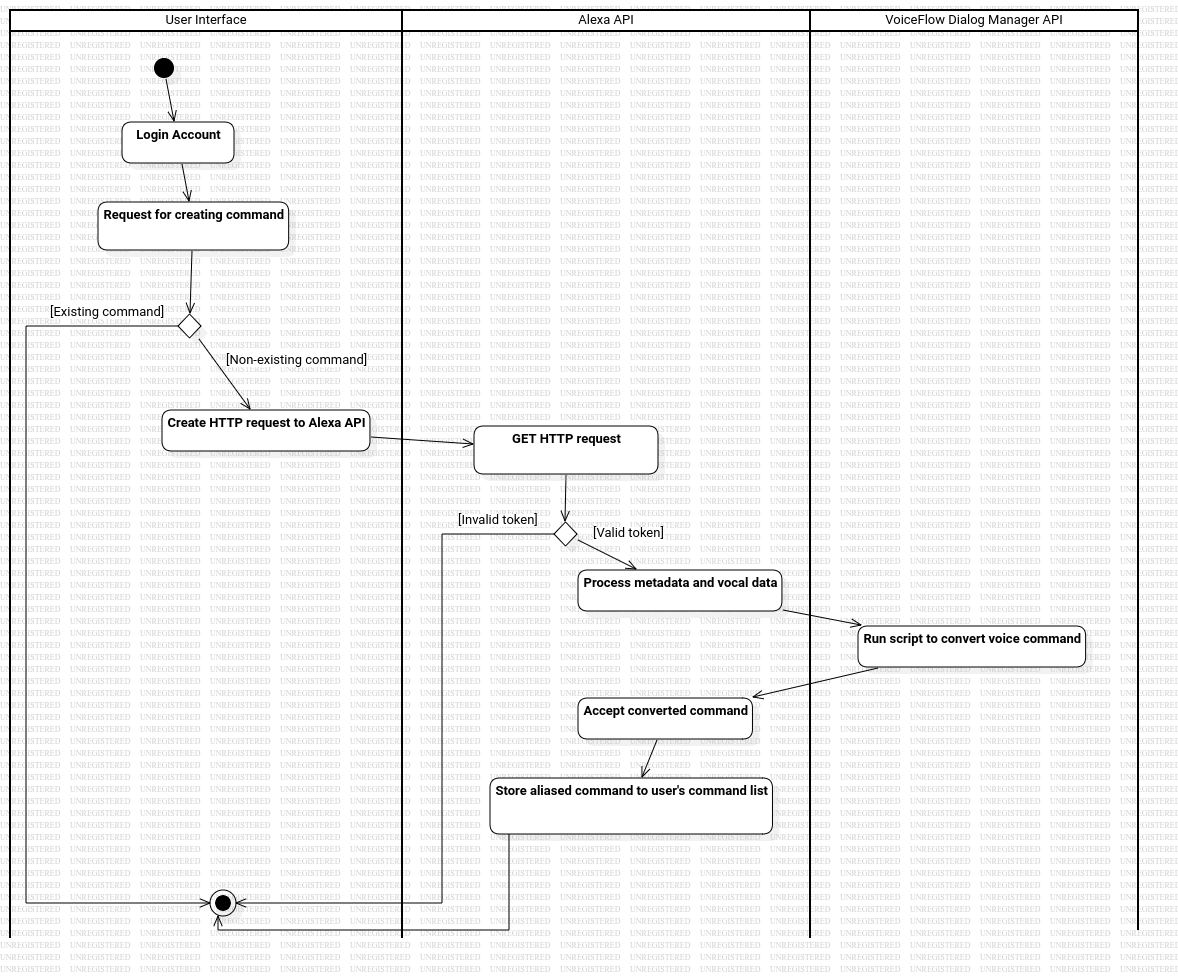
\includegraphics[width=1\textwidth]{Figures/SuggestedActivityDiagram.png}
    \caption{Activity Diagram for Voice Command Pipeline}\label{fig:suggested_activity}
\end{figure}





\section{Functional View}

\subsection{Stakeholders’ uses of this view}

The Functional View offers an overview of how architectural elements work together to provide the various functionalities of FarmBot. Below, you can find the FarmBot Stakeholders' uses of this view:
\begin{itemize}
    \item \textbf{Developers}: The developers' main concern is the quality of design and the internal structure of the FarmBot system. The internal structure is crucial to meet the desired quality requirements such as availability, ability to scale, security during development. Also developers can use this view to see the external interfaces.
    \item \textbf{End Users} (Students, Researchers, Home Users, Artwork Creators): End users can use this view to learn the functionalities provided by FarmBot and how they are provided, what external interfaces are used.
    \item \textbf{Ministry of Agriculture}: Their use of this view is to have a more in-depth knowledge of the overall system, internal structure, external interfaces, and functionality for auditing.
\end{itemize}

\subsection{Component Diagram}

\begin{figure}[H]
    \centering
    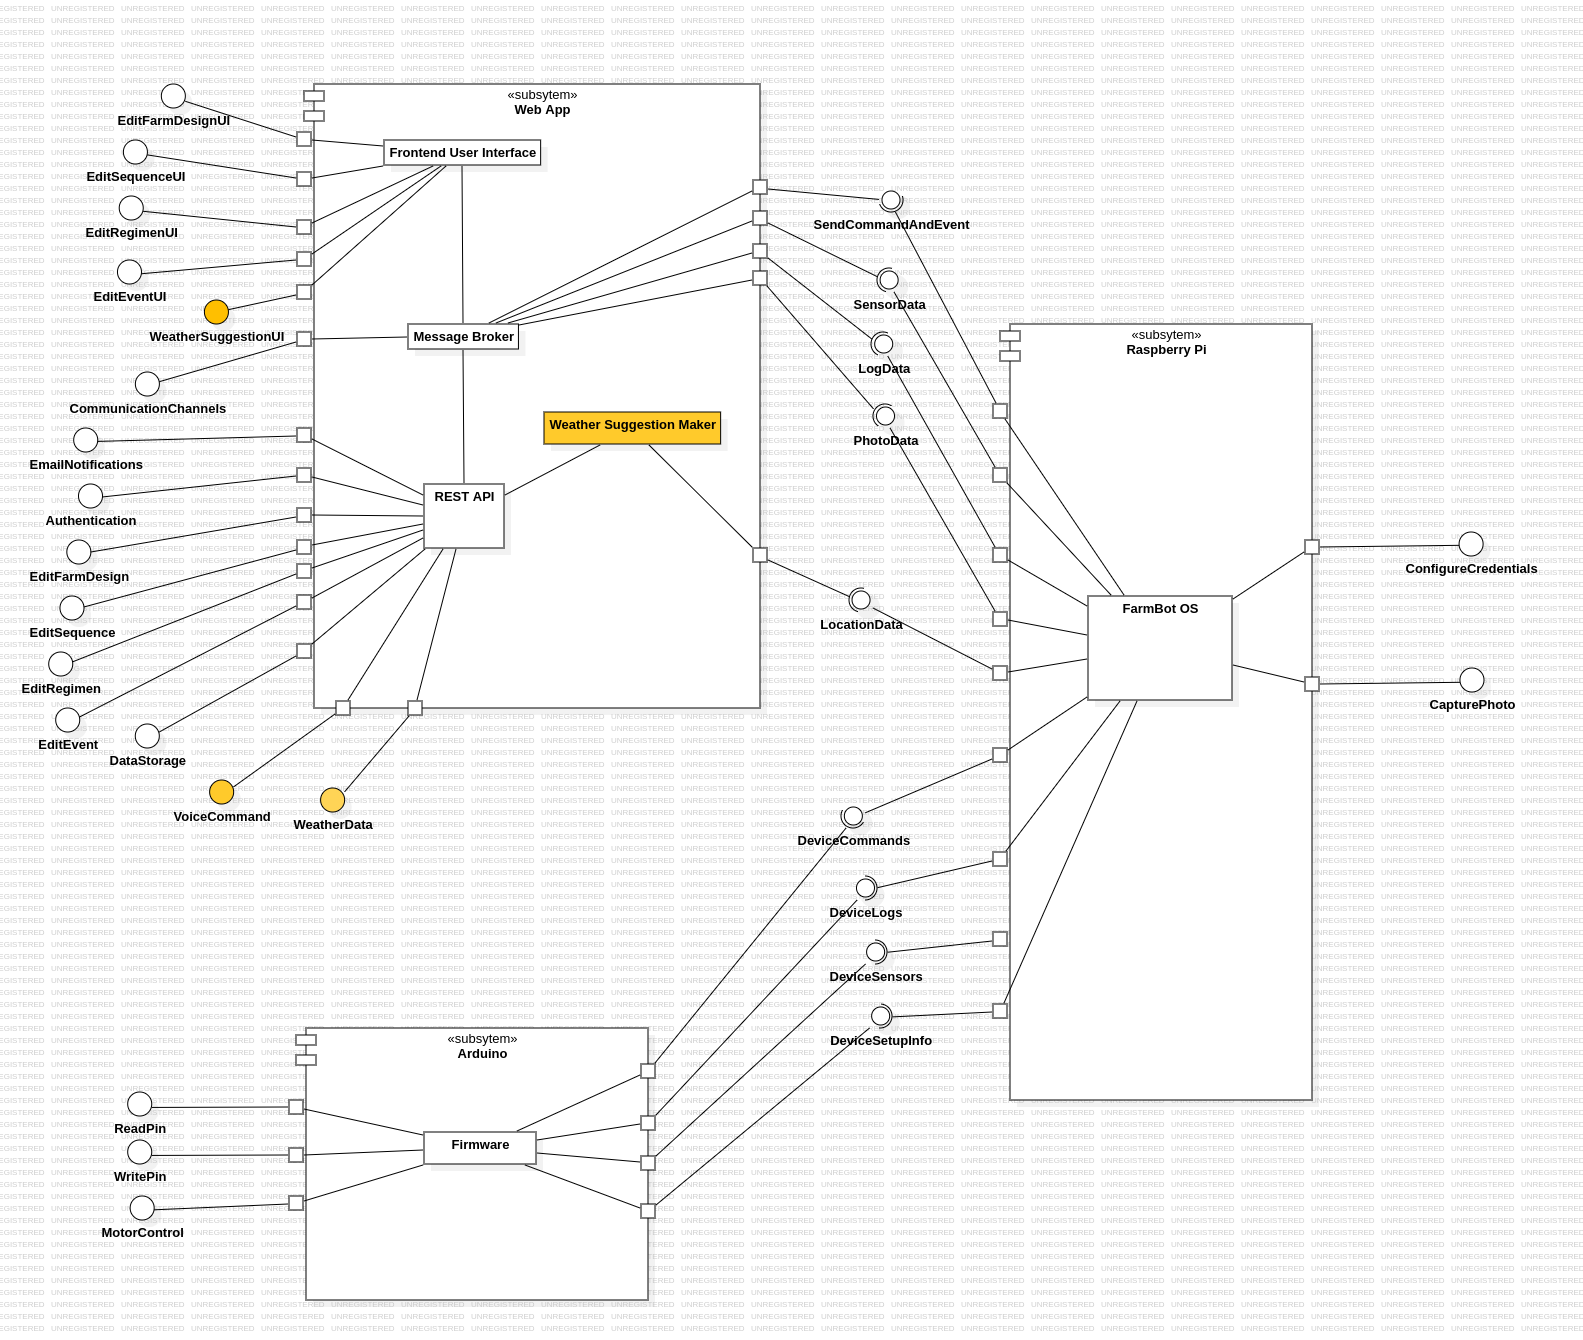
\includegraphics[width=1\textwidth]{Figures/ComponentDiagramSuggestions.png}
    \caption{Suggested Component Diagram for FarmBot}\label{fig:suggested_component_diagram}
\end{figure}

The suggested component diagram for FarmBot extends the original one with three external interfaces, a part inside the web app which makes the suggestions based on weather and a interface between FarmBot device to gather the device location. The Frontend User Interface provides an external interface for the user to add voice commands. The REST API provides two external APIs for voice commands and weather data respectively. Voice commands are processed and extracted using external services. Therefore, the interaction between these services are provided through this API. Lastly, the weather data interface allows the web app to communicate with the external weather service providers.

\subsection{Internal Interfaces}

\begin{figure}[H]
    \centering
    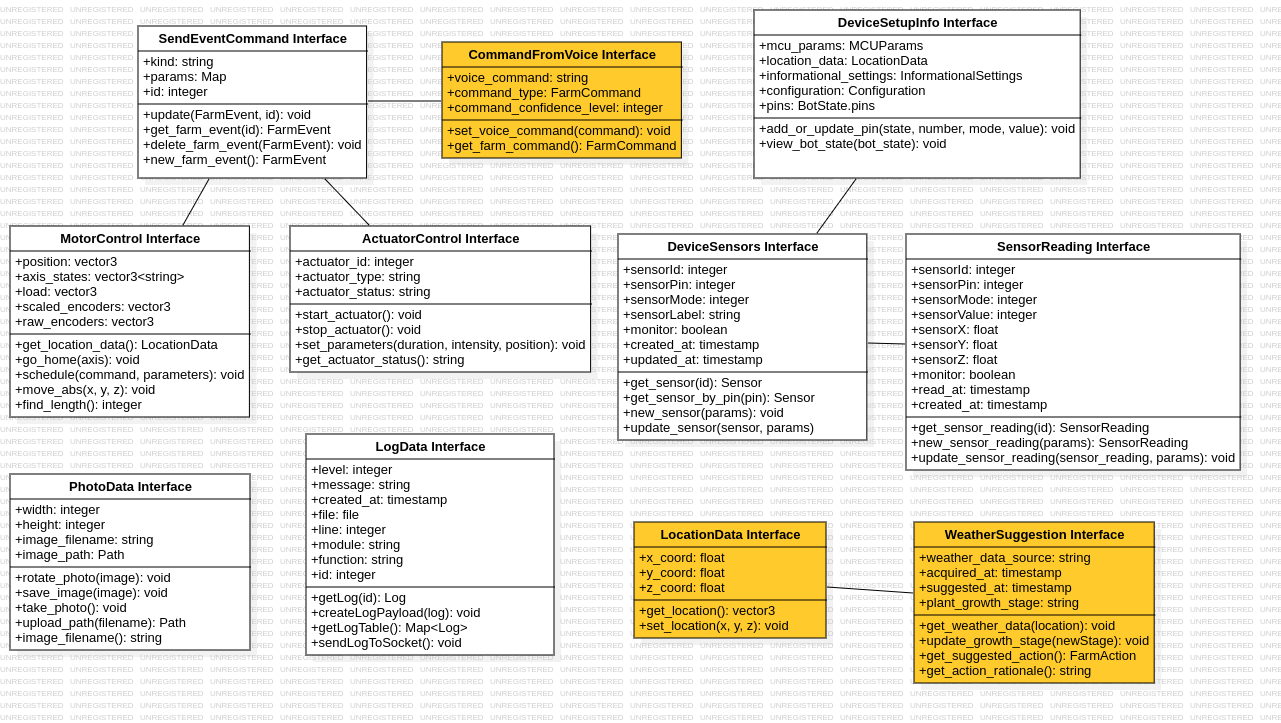
\includegraphics[width=1\textwidth]{Figures/Internal_Interface_Diagram_Suggestions.png}
    \caption{Suggested Internal Interfaces Diagram for FarmBot}\label{fig:internal_interfaces_diagram_suggestions}
\end{figure}

\begin{itemize}
    \item \textbf{CommandFromVoice Interface:} \begin{itemize}
        \item \textbf{voice\_command}: The recognized text of voice command.
        \item \textbf{command\_type}: The type of the command such as WATERING, PLANTING, SCANNING\_FOR\_WEEDS
        \item \textbf{command\_confidence}: The level of confidence for the recognized text of voice command, acquired from external service Voiceflow.
        \item \textbf{set\_voice\_command(command)}: Sets the recognized voice command and the type of it.
        \item \textbf{get\_farm\_command()}: Returns the FarmCommand to be executed
    \end{itemize}
    \item \textbf{LocationData Interface:} \begin{itemize}
        \item \textbf{x\_coord}: X coordinate of the FarmBot device
        \item \textbf{y\_coord}: Y coordinate of the FarmBot device
        \item \textbf{z\_coord}: Z coordinate of the FarmBot device
        \item \textbf{get\_location()}: Returns a three dimensional vector storing the coordinates of FarmBot device
        \item \textbf{set\_location(x, y, z)}: Updates the current coordinates of FarmBot device with the given parameters 
    \end{itemize}
    \item \textbf{WeatherSuggestion Interface:} \begin{itemize}
        \item \textbf{weather\_data\_source}: Specifies the source of the weather data
        \item \textbf{acquired\_at}: The timestamp when latest weather data was acquired
        \item \textbf{suggested\_at}: The timestamp when suggestion was made
        \item \textbf{plant\_growth\_stage}: Specifies the current growth stage of the plants being cultivated by the FarmBot (e.g., seedling, vegetative, flowering).
        \item \textbf{get\_weather\_data(location)}: Acquires the current weather data through the REST API.
        \item \textbf{update\_growth\_stage(newStage)}: Updates the growth stage according to the crop information
        \item \textbf{get\_suggested\_action()}: Returns a FarmAction that is computed by taking into account the current weather data and the growth stage of the crop
        \item \textbf{get\_action\_rationale()}: Returns a human friendly string of rationale, to be displayed to the user, explaining the suggested action
    \end{itemize}
\end{itemize}

\subsection{Interaction Patterns}

\begin{figure}[H]
    \centering
    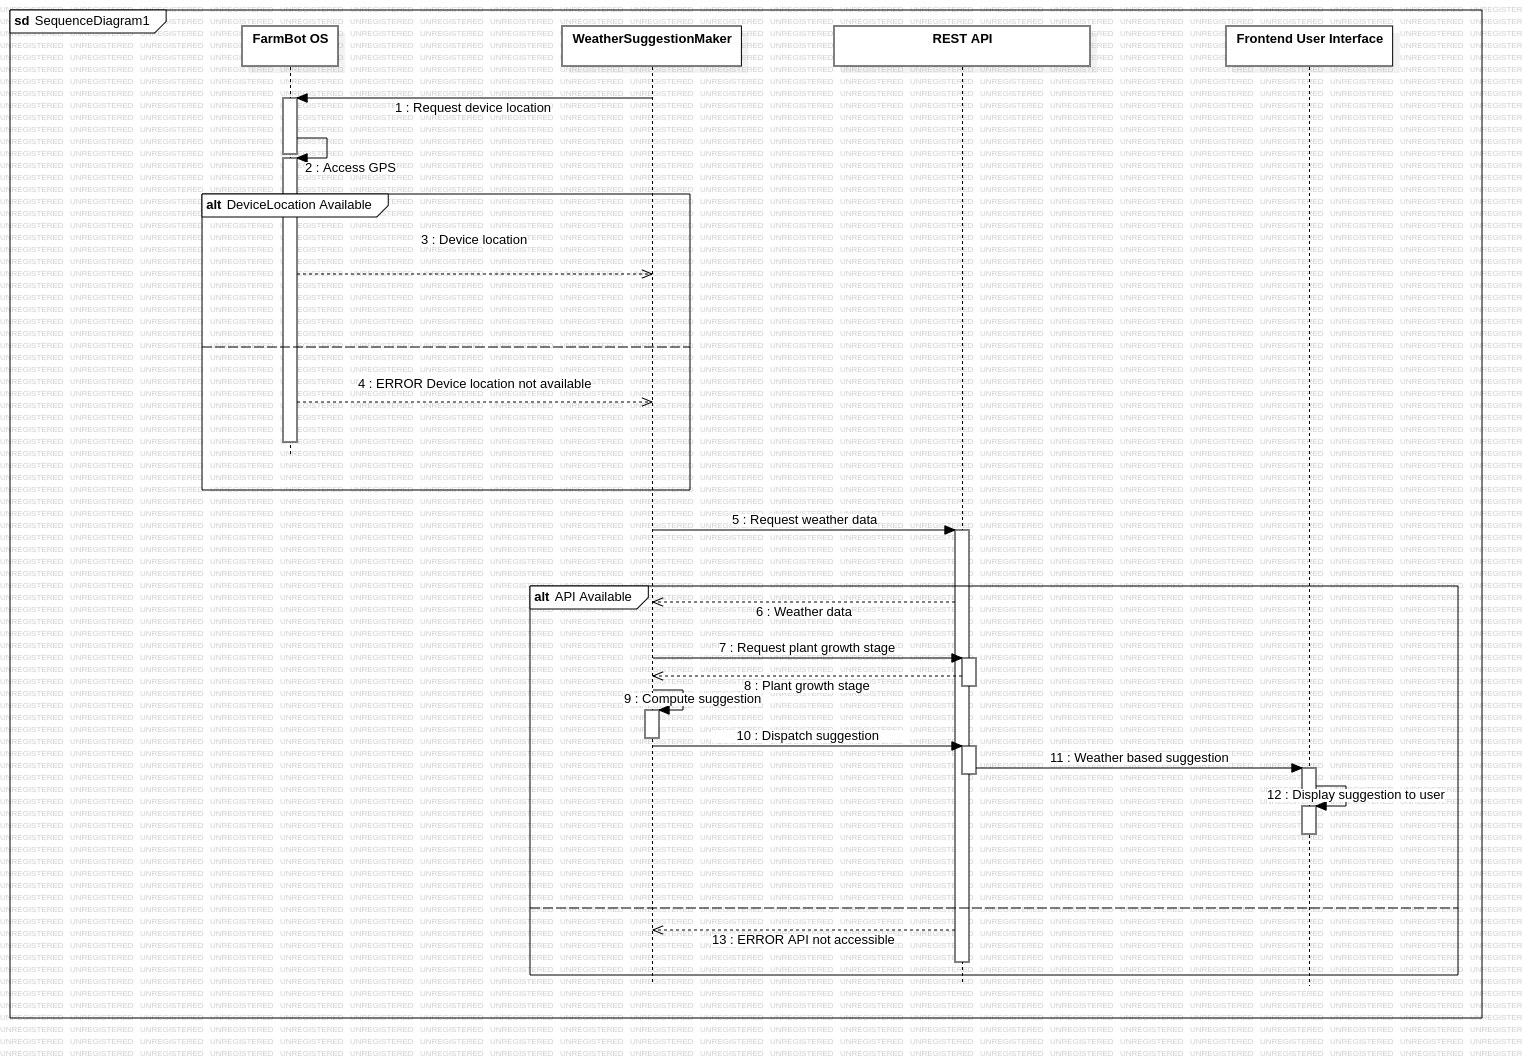
\includegraphics[width=1\textwidth]{Figures/SequenceDiagramSuggestions.png}
    \caption{Sequence Diagram for Weather Based Suggestion of FarmBot}\label{fig:sequence_diagram_suggestions}
\end{figure}

The sequence diagram in Figure 5.5, shows the weather based suggestion of FarmBot. WeatherSuggestionMaker, requests current location data from FarmBot OS. FarmBot OS, access the GPS device and returns the location data to the WeatherSuggestionMaker or in case of failure returns an error. Consequently, WeatherSuggestionMaker requests weather data from the REST API using the location data it acquired. The REST API returns the weather data, after that another request for growth stage of plant is made. Using these data, WeatherSuggestionMaker computes a suggestion and dispatches it to the web app through the REST API. Frontend User Interface displays it to the user. In the case that the API is not available, an error is returned with the requests.

\section{Information View}

\subsection{Stakeholders’ uses of this view}

The key use of the \textbf{Information View} for the stakeholders of FarmBot is to ensure that the data requirements are correctly understood and that the data is stored and handled correctly. The different stakeholders' uses of this view are as follows:
\begin{itemize}
    \item \textbf{End users:} The end users primarily interact with the information view to understand the data being collected by FarmBot and how it relates to their gardening activities. They may use this view to monitor plant health, track growth progress, and receive alerts or recommendations.
    \item \textbf{Developers:} Developers use the information view to design and implement features related to data collection, storage, and processing. They ensure that the data is collected efficiently, stored securely, and can be accessed and manipulated as needed for various functionalities.
    \item \textbf{Ministry of Agriculture:} The Ministry of Agriculture utilizes the information view to oversee and regulate the use of FarmBot data for agricultural purposes. They may use this view to monitor farming practices, analyze trends, and make informed decisions regarding agricultural policies and practices.
\end{itemize}

\subsection{Database Class Diagram}

% \textbf{Database Class Diagram} involving the key database or main memory objects \textbf{for your suggestions.} Complete with relevant associations. Descriptions of the non-obvious names (for classes, attributes, operations) should also be given.
\begin{figure}[H]
    \centering
    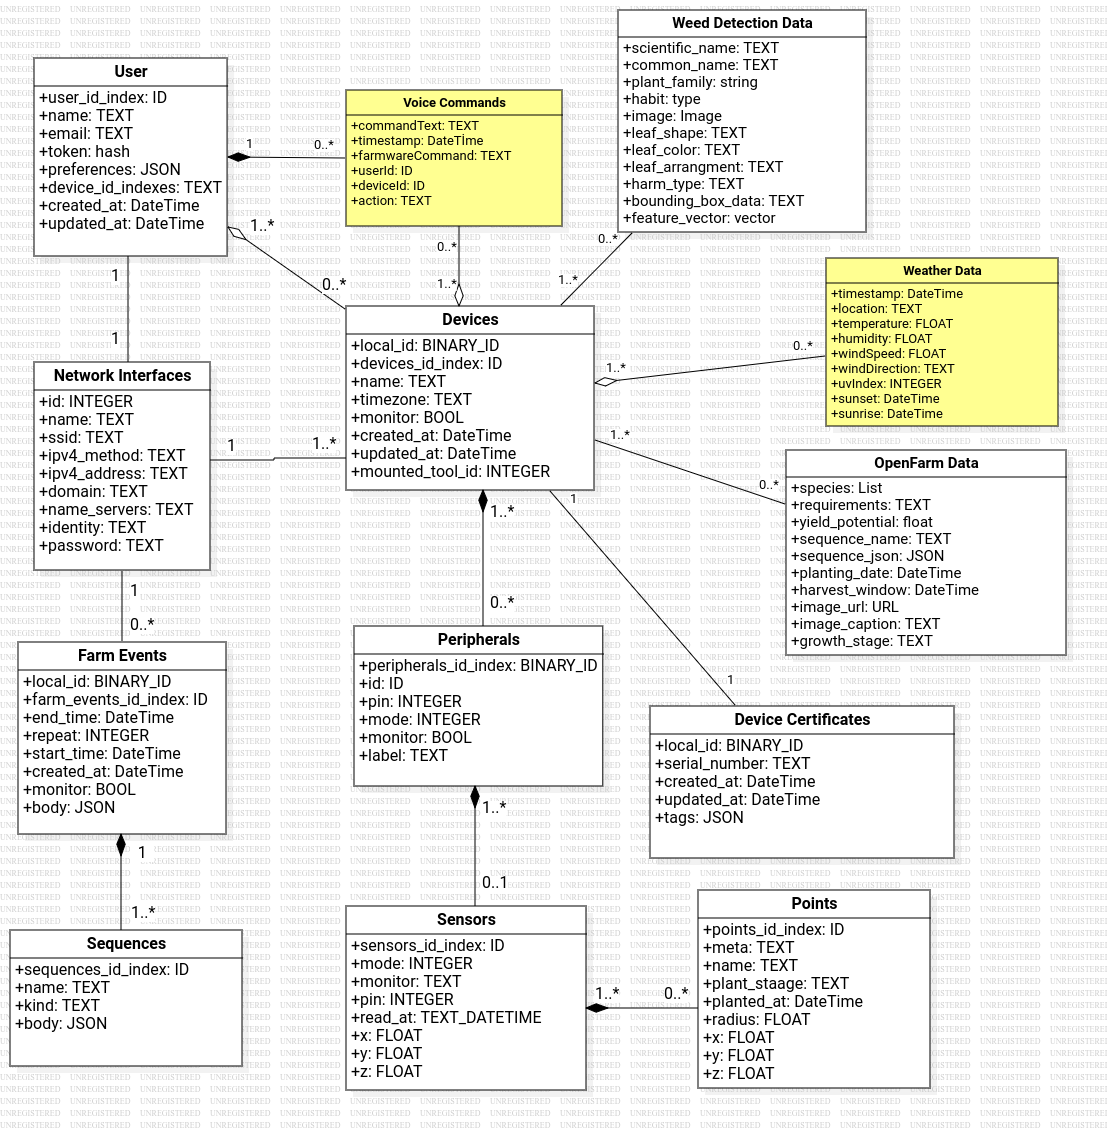
\includegraphics[width=1\textwidth]{Figures/SuggestedDBDiagram.png}
    \caption{Suggested Database Class Diagram for FarmBot}\label{fig:suggested_database}
\end{figure}

The suggested database class diagram for FarmBot is shown in Figure~\ref{fig:suggested_database}. The diagram shows the key database objects of the system. It now includes \textbf{Weather Data} and \textbf{Voice Command} as new database objects of the system.

\begin{itemize}
    \item \textbf{Weather Data:} This object stores the weather information of the FarmBot location. Using the location information, the interface fetches the current temperature, humidity, and weather conditions from the Local Weather API. The related data is also stored in this object for future use, such as predicting the weather conditions for the upcoming days and adjusting the FarmBot's schedule accordingly.
    \item \textbf{Voice Command:} This object stores the voice commands of the users processed by the VoiceFlow API. This table has columns for storing voice command data, such as command text and the corresponding action to be executed by the FarmBot system. The voice commands are used to control the FarmBot using voice commands through the Alexa API.
\end{itemize}

\subsection{Operations on Data}
% Descriptions of the operations are given in the database class diagram. These operations may deal with the storage and handling of information regarding stores, customers, products, and so on. \textbf{Operations for your suggestion should be listed in a table or using bullets.}
% These usually include CRUD (Create Read Update Delete) operations.

\begin{table}[H]
    \centering
    \begin{tabular}{|c|c|c|}
        \hline
        \textbf{Operation} & \textbf{Description}                     & \textbf{Object} \\
        \hline
        CreateWeatherData  & Creates a new weather data object        & Weather Data    \\
        \hline
        ReadWeatherData    & Reads the weather data of the location   & Weather Data    \\
        \hline
        UpdateWeatherData  & Updates the weather data of the location & Weather Data    \\
        \hline
        DeleteWeatherData  & Deletes the weather data of the location & Weather Data    \\
        \hline
        CreateVoiceCommand & Creates a new voice command object       & Voice Command   \\
        \hline
        ReadVoiceCommand   & Reads the voice command data             & Voice Command   \\
        \hline
        UpdateVoiceCommand & Updates the voice command data           & Voice Command   \\
        \hline
        DeleteVoiceCommand & Deletes the voice command data           & Voice Command   \\
        \hline
    \end{tabular}
    \caption{CRUD Operations on the Suggested System}\label{tab:operations_on_data}
\end{table}

Some of the operations on data for FarmBot are listed in Table~\ref{tab:operations_on_data}. These operations include CRUD (Create, Read, Update, Delete) operations for the Weather Data and Voice Command objects. The operations are used to create, read, update, and delete the system's weather data and voice command data. The operations are related to other objects as mentioned in Table~\ref{tab:crud_operations}.

\section{Deployment View}

%Refer to \textit{R\&W Chapter 21}.

\subsection{Stakeholders’ uses of this view}

The stakeholders uses of the Deployment view are described as follows:
\begin{itemize}
    \item Developers: They use this view to better understand how they should orchestrate their development environment, what should their coverage be for deployment.
    \item End Users: They use this view to learn what tools, software or applications they need to get the system up and running.
    \item Ministry of Agriculture: They use this view to better understand dependencies, relations and interactions in the system. It can offer a inside view to how the system is orchestrated, aiding them in auditing.
\end{itemize}


\subsection{Deployment Diagram}

\begin{figure}[H]
    \centering
    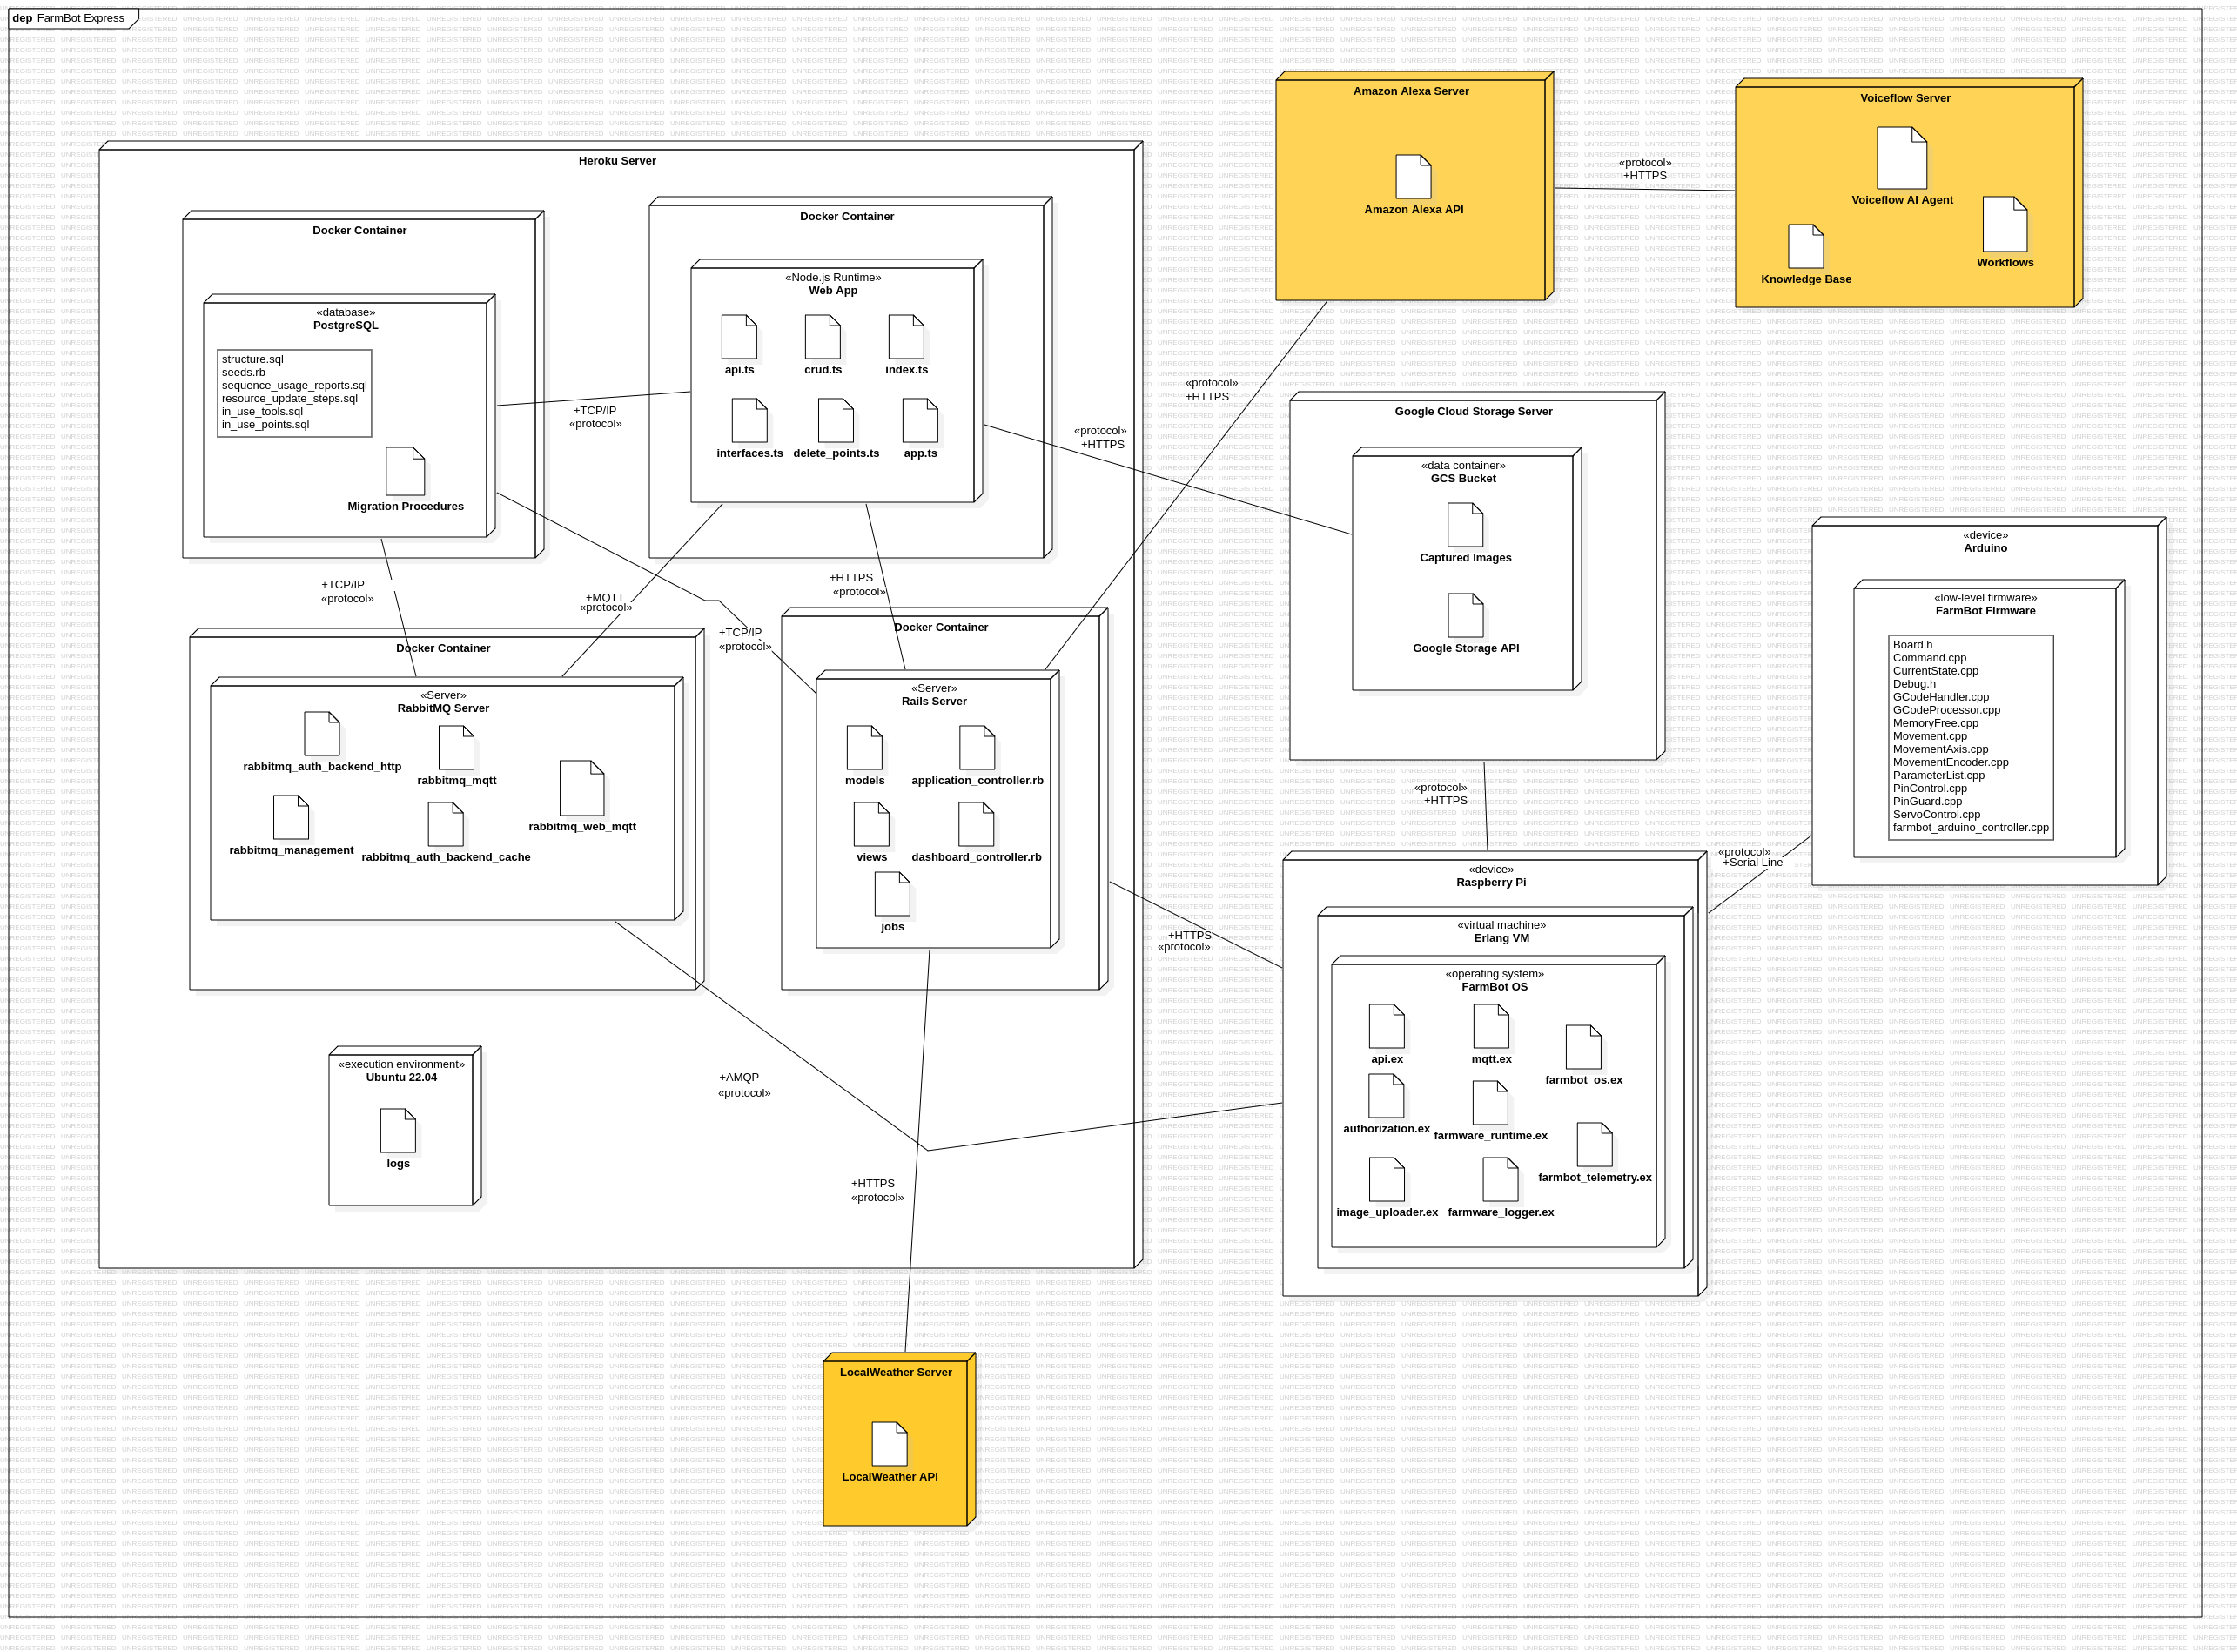
\includegraphics[width=1\textwidth]{Figures/DeploymentDiagramSuggestions.png}
    \caption{Suggested Deployment Diagram for FarmBot}\label{fig:deployment_diagram_suggestions}
\end{figure}

The deployment diagram for the suggestions extends the original deployment diagram with three nodes. These are the Amazon Alexa servers used for capturing the voice and the Voiceflow servers for processing the voice to acquire the command. For the weather feature, a node for the LocalWeather Servers is added to the diagram. This node holds the LocalWeather API artifact. The REST API interacts with this server to acquire the weather data for the day and use it to make suggestions based on it. 

\section{Design Rationale}
% State \textbf{one rationale} specifically referring to each view presented \textbf{for your suggestions.}
\begin{itemize}
    \item \textbf{Context View:} The suggested context view includes the Local Weather API and Alexa API as new external system entities.
          \begin{itemize}
              \item Local Weather API: Integrating the Local Weather API into the context view allows the FarmBot system to adapt its operations based on real-time weather conditions. This improves automation by enabling the FarmBot to adjust watering schedules, activate frost protection measures, or optimize growth lamp usage based on temperature, humidity, and precipitation data.
              \item Alexa API: The inclusion of the Alexa API in the context view facilitates voice-controlled interaction with the FarmBot. This enhances user experience by providing a more intuitive and hands-free way to control the system. Users can issue commands to perform actions like starting/stopping irrigation, adjusting nutrient delivery, or receiving status updates using simple voice prompts.
          \end{itemize}
    \item \textbf{Functional View:} \begin{itemize}
        \item Weather Suggestions: An internal interface for the location data is used for the operation of the weather based suggestions internal interface. This suggestion interface is used for acquiring weather data from REST API and computing a farm action to be taken based on the current status. Seperation of concerns is achieved and interface segregation leads to better maintainability.
        \item Voice Commands: A seperate internal interface for commands is added following the interface segregation principle. This interface keeps additional data for the captured voice and recognized command. The confidence score can be used to decide whether executing or not.
    \end{itemize}
    \item \textbf{Information View:}
          \begin{itemize}
              \item Weather Data: Integrating the Local Weather API expands the information view by providing real-time weather data alongside existing FarmBot sensor readings. This comprehensive view allows for a more holistic understanding of the farm environment. Users can easily correlate sensor data with weather conditions to identify potential issues or optimize growing conditions. Database stores the necessary information that users can access and analyze the weather data.
              \item Voice Command: The inclusion of the Alexa API in the information view offers the ability to display voice command options directly within the FarmBot interface. To support user customization, the FarmBot system will need to store data related to user-defined aliases, favorite commands, and potentially custom command sets. The information view ensures that the user can easily understand the stored voice commands and their corresponding actions.
          \end{itemize}
    \item \textbf{Deployment View:} \begin{itemize}
        \item LocalWeather API: This is an external service provided by an external service provider. Therefore, the app must interact with it over the network. This interaction follows a request-response pattern since for each day, the web-app makes a request to acquire the weather data and gets the weather data in response. Therefore, the app interacts with the Local Weather API through the Rails server REST API.
        \item Voice Command: The voice commands require two external services, Amazon Alexa and Voiceflow. By using these external services, the complexity of FarmBot project is minimized. It provides better maintainability. In addition, since these services are not on FarmBot servers, they cost less to scale. Providing better availability. Commands are acquired through the REST API and sent over to the physical FarmBot device via the MQTT.
    \end{itemize}
\end{itemize}